% submit to https://sites.google.com/site/wpmvp2014/home
\documentclass[10pt]{sigplanconf}

% The following \documentclass options may be useful:

% preprint      Remove this option only once the paper is in final form.
% 10pt          To set in 10-point type instead of 9-point.
% 11pt          To set in 11-point type instead of 9-point.
% authoryear    To obtain author/year citation style instead of numeric.

\usepackage{amsmath}
\usepackage{listings}
\usepackage{hyperref}

\special{papersize=8.5in,11in}
\setlength{\pdfpageheight}{\paperheight}
\setlength{\pdfpagewidth}{\paperwidth}

\conferenceinfo{WPMVP '14}{February 16, 2014, Orlando, FL, USA} 
\copyrightyear{2014} 
\copyrightdata{978-1-4503-2653-7/14/02}
\doi{2568058.2568060}

\lstset{captionpos=b, float}

\usepackage{tikz}
\usetikzlibrary{positioning}
\usetikzlibrary{shadows}
\usetikzlibrary{arrows}
\usetikzlibrary{shapes}

\providecommand{\boostsimd}{\textsc{Boost.SIMD}}
\providecommand{\cpp}[1][~]{\textsc{C++}#1}
\providecommand{\ie}[1][~]{\textit{i.e.}#1}
\providecommand{\eg}[1][~]{\textit{e.g.#1}}


\begin{document}


\title{Exploring the Vectorization of Python Constructs Using Pythran and Boost SIMD}

\authorinfo{Serge Guelton}
           {QuarksLab, T{\'e}l{\'e}com Bretagne}
           {sguelton@quarkslab.com}
\authorinfo{Jo{\"e}l Falcou}
           {LRI, Universit\'e Paris-Sud}
           {joel.falcou@lri.fr}
\authorinfo{Pierrick Brunet}
           {INRIA/MOAIS}
           {pierrick.brunet@inria.fr}

\maketitle

\begin{abstract}

    The Python language is highly dynamic, most notably due to late binding. As
    a consequence, programs using Python typically run an order of magnitude
    slower than their C counterpart. It is also a high level language whose
    semantic can be made more static without much change from a user point of
    view in the case of mathematical applications. In that case, the language
    provides several vectorization opportunities that are studied in this
    paper, and evaluated in the context of Pythran, an ahead-of-time compiler
    that turns Python module into C++ meta-programs.

\end{abstract}

%\category{CR-number}{subcategory}{third-level}

% general terms are not compulsory anymore, 
% you may leave them out
%\terms
%term1, term2

\keywords
Vectorization, Meta-Programming, Python, C++


%%
%%
\section{Python, Unboxing and Pythran}

The Python language~\cite{rossum97} has grown in audience for the past ten
years, even reaching the world of scientific computations~\cite{oliphant2007}
thanks to the \texttt{numpy} module~\cite{numpyarray2011}, a module that
provides an efficient multi-dimensional array type, and the \texttt{scipy}
package~\cite{scipy} that provides a MATLAB-like API. As a consequence, more
and more code is being written either in pure Python, generally to prototype an
application, or as a Python and native code mix when performance matters.
However, Python trades performance for dynamicity and does not particularly
shines in terms of performance.

\subsection{Python Performance Shortcomings}

To illustrate the relatively bad performance of Python for numerical
computations, let us consider the sixth problem from the Project Euler: ``Find
the difference between the sum of the squares of the first one hundred natural
numbers and the square of the sum``. A straight-forward solution can be coded
as in Listing~\ref{lst:euler06-py} in Python or as in
Listing~\ref{lst:euler06-c} in C. A comparison of the performance of the Python
function and the C function called through the \texttt{ctypes} module shows
that the C version runs more than $\times250$ faster than the Python version.
Enabling compiler auto-vectorization even makes the C version $\times400$
faster than the Python version (Note that to perform more reliable time
measurements, the size of the problem has been increased to 100001 instead of
101).

There are two main reasons for the poor performance of Python:

\begin{description}

    \item[dynamic binding] each variable access is made through a dictionary
        look-up that binds variable names to variable instances;

    \item[boxing] each variable value is encapsulated into a heap-allocated
        generic object ---the \texttt{PyObject}--- which implies extra
        indirections for each operation.

\end{description}

In that context, it does not make sense to speak about vectorization: the
nature of an operation is unknown to the interpreter until its execution, and
data are not even contiguous in memory.

\lstinputlisting[language=python, label={lst:euler06-py}, caption={Solution to the Project Euler Sixth Problem in Python}]{experiments/euler06.py}

\lstinputlisting[language=c, label={lst:euler06-c}, caption={Solution to the Project Euler Sixth Problem in C}]{experiments/euler06.c}


\subsection{Compiling Python Code}

Several approaches have been proposed to solve the performance issue of Python:
using native modules, relying on Ahead-Of-Time (AOT) compilation or
Just-In-Time (JIT) compilation.

A native module is a shared library whose interface makes it callable from the
Python interpreter using the regular \texttt{import} mechanism. It makes it
possible to call native code from Python in a transparent way. Typically Python
objects are unboxed when transfered from Python to C, where efficient
computations can happen. Then the result is boxed when getting back to the
Python world. In between, vectorization can happen. This is the approach taken
by the \texttt{numpy} module: a native type, the \texttt{ndarray} contains
contiguous unboxed elements, say single precision floating point numbers, and
provides a great deal of high-level functions to manipulate them. All the
computation-intensive part is done in pure C.  Vectorization can eventually
happen at this level, for instance when performing a point-to-point operation
like the sum of two arrays. However the granularity of the operations limits
the ratio of \texttt{load}/\texttt{store} versus operation. For instance, if
\texttt{a}, \texttt{b} and \texttt{c} are 1-D arrays, the sum \texttt{a + b +
c} is computed using two loops and an intermediate array. It means there are 4
\texttt{load}/\texttt{store} and only two additions per loop iteration and vectorization is
unlikely to be profitable.

AOT compilation uses type inference or type annotation to statically compute
the type of all (like in Shedskin~\cite{shedskin2006},
Parakeet~\cite{parakeet2012}) or part of (like in Cython~\cite{cython2010} or
Numba~\cite{numba}) variables, effectively unboxing them to speed-up
computations. Using JIT compilation, type information is available at runtime
and the unboxing decision is based on profitability, e.g.\ according to a trace
analysis. This is the approach of the PyPy project~\cite{pypy2009}. In both
cases, generation of vector instruction is possible, but none of the cited
project uses it. Indeed automatic vectorization is a complex topic, and as
stated in~\cite{maleki2011}, many cases are not yet correctly supported even
for mainstream C/C++/FORTRAN compilers.

\subsection{The Pythran Compiler}

Pythran~\cite{pythran2013, pyhpc2013} is also an AOT compiler, but it holds the
unique property of turning Python modules into C++11 \emph{meta-programs}. It
does not need any type annotations during translation and keeps the
polymorphism of original functions, respecting Python's duck typing. Its
compilation work-flow is described in Figure~\ref{fig:pythran-compiler}: Python
source is turned into generic C++11 code that is then instantiated for the
given types provided as extra annotations.  Like other AOT compilers, it
unboxes all variables for better performance, but also performs a wide variety
of optimizations such as lazy evaluation, constant folding, expression fusion
etc.  It supports core \texttt{numpy} constructs and most Python constructs, to
the notable exception of user classes. Instructions such as \texttt{eval},
\texttt{exec} or \texttt{getattr} are not supported either.

\begin{figure}

\centering
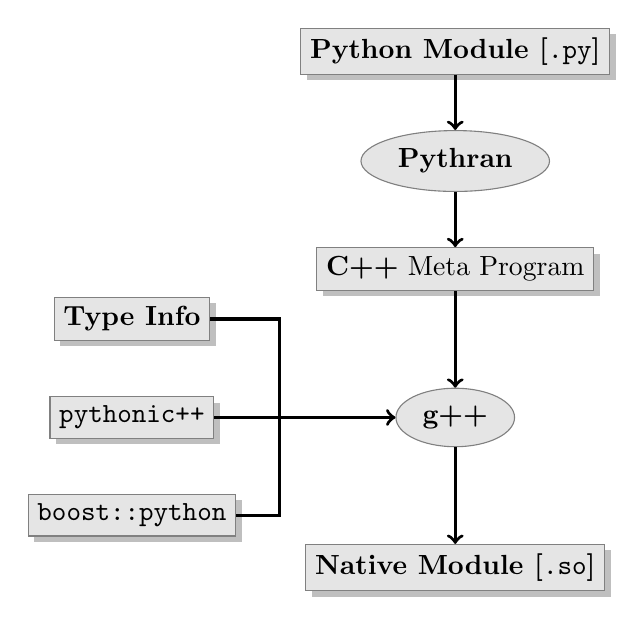
\begin{tikzpicture}[
file/.style={draw=black!50,fill=black!10,rectangle, drop shadow, align=center,
node distance=0.7cm},
    tool/.style={draw=black!50,fill=black!10,ellipse, align=center, node
    distance=0.7cm}]
    \node[file] (python) {\textbf{Python Module [\texttt{.py}]}};
    \node[tool] (pythran) [below=of python] {\textbf{Pythran}};
    \node[file] (meta-cxx) [below=of pythran] {\textbf{C++} Meta Program};
    \node[tool] (gxx) [yshift=-1.5em, below=of meta-cxx] {\textbf{g++}};
    \node (empty) [xshift=-1em, left=of gxx] {};
    \node[file] (pythonic) [left=of empty] {\textbf{\texttt{pythonic++}}};
    \node[file] (annotation)     [above=of pythonic] {\textbf{Type Info}};
    \node[file] (boost) [below=of pythonic] {\textbf{\texttt{boost::python}}};
    \node[file] (so) [yshift=-1.5em, below=of gxx] {\textbf{Native Module
    [\texttt{.so}]}};

\draw[very thick, ->] (python) -- (pythran);
\draw[very thick] (annotation) -| (empty.center);
\draw[very thick, ->] (pythran) -- (meta-cxx);
\draw[very thick, ->] (meta-cxx) -- (gxx);
\draw[very thick] (boost) -| (empty.center);
\draw[very thick, ->] (pythonic) -- (gxx);
\draw[very thick, ->] (gxx) -- (so);
\end{tikzpicture}

\caption{Pythran compiler work-flow.}
\label{fig:pythran-compiler}
\end{figure}


This paper explores the vectorization of Python programs based on the idea that
many Python constructs already exhibit good vectorization opportunities. Thus
the goal of the compiler switches from automatic vectorization to vectorization
of high-level Python intrinsics. One of the difficulties of vectorizing Python
functions is linked to function polymorphism: vectorization in the context of
C++ meta-programs is first examined in Section~\ref{sec:meta-vectorization},
and Python constructs that can benefit from vectorization are then described in
Section~\ref{sec:python-semantic}. The approach is validated using the Pythran
compiler on several kernels presented in Section~\ref{sec:benchs}.

%%
%%
\section{Vectorization of a Meta-Program}
\label{sec:meta-vectorization}

Single Instruction Multiple Data (SIMD) extensions have been a feature of
choice for processor manufacturers for a couple of decades. However,
programming applications that take advantage of the SIMD extension available on
the current target remains a complex task. Programmers that use low-level
intrinsics have to deal with a verbose programming style due to the fact that
SIMD instructions sets cover a few common functionalities, requiring to bury
the initial algorithms in architecture specific implementation details.
Furthermore, these efforts have to be repeated for every different extension
that one may want to support, making design and maintenance of such
applications very time consuming. 

\boostsimd{} is a high-level C++ library to program SIMD architectures. 
Designed as an \textit{Embedded Domain Specific Language}, \boostsimd{} 
provides both expressiveness and performance by using generic programming 
to handle vectorization. \boostsimd{} does not only provide a portable 
way but also enables the use of common programming idioms when designing 
SIMD-aware algorithms. Two components are provided:

\begin{itemize}
\item \textbf{An abstraction of SIMD registers} for portable algorithm design,
coupled with a large set of functions covering the classical set of operators
along with a sensible amount (200+) of mathematical functions and utility functions,
\item \textbf{A support for \cpp standard components} like \texttt{Iterator}
over SIMD \texttt{Range}, SIMD-aware allocators and SIMD-aware STL algorithms.
\end{itemize}

\subsection{SIMD register abstraction}
The first level of abstraction introduced by \textsc{Boost.} \textsc{SIMD} is
the \texttt{pack} class. For a given type \texttt{T} and a given static integral 
value \texttt{N} (\texttt{N} being a power of 2), a \texttt{pack} encapsulates
the best type able to store a sequence of \texttt{N} elements of type \texttt{T}.
For arbitrary \texttt{T} and \texttt{N}, this type is simply \texttt{std::array<T,N>}
but when \texttt{T} and \texttt{N} matches the type and width of a SIMD register,
the architecture-specific type used to represent this register is used instead.
This semantic provides a way to use arbitrarily large SIMD registers on any system
and let the library select the best vectorizable type to handle them. By default,
if \texttt{N} is not provided, \texttt{pack} will automatically select a value
that will trigger the selection of the native SIMD register type. Moreover, by
carrying informations about its underlying scalar type, \texttt{pack} enables
proper instruction selection even when used on extensions (like SSE2 and above)
that map all integral type to a single SIMD type (\texttt{\_\_m128i} for SSE2).\\

\texttt{pack} handles these low-level SIMD register type as regular objects with
value semantics, which includes the ability to be constructed or copied from a
single scalar value, list of scalar values, iterator or range. In each case, the
proper register loading strategy (splat, set, load or gather) will be issued.
\texttt{pack} also takes care of issues like boolean predicates support and provides
both a range and a tuple-like interface.

\subsection{Interaction with Standard Algorithm}
Modern \cpp programming style based on Generic Programming usually leads to an
intensive use of various STL components like Iterators. \boostsimd{} provides
iterator adaptors that turn regular random access iterators into iterators
suitable for SIMD processing. These adaptors act as free functions taking
regular iterators as parameters and return iterators that output \texttt{pack}
whenever dereferenced. These iterators are then usable directly in usual STL
algorithms such as \texttt{transform} or \texttt{fold} (Listing \ref{lst:tl_example}).

\begin{lstlisting}[language=c++, label={lst:stl_example}, caption={SIMD Iterator with STL algorithm},label=stl_example]
std::vector<int,allocator<int>> v(N),r(N);
std::transform (
 simd::begin(v.begin()),simd::end(v.end()),
 simd::begin(r.begin()),
 [](pack<int> const& p) { return p*p; } 
);
\end{lstlisting}

Previous examples of integration within standard algorithm are still limited.
Applying \texttt{transform} or \texttt{fold} algorithm on SIMD aware data
requires the size of the data to be an exact multiple of the SIMD register width
and, in the case of fold, to potentially perform additional operations at the
end of its call. To alleviate this limitation, \boostsimd{}
provides its own overload for both \texttt{transform} and \texttt{fold} that take
care of potential trailing data and performs proper completion of \texttt{fold}.
Moreover, as \boostsimd{} provides default implementation of all its function for scalar values,
we can rely on polymorphic callable object to write a mixed scalar/SIMD call to algorithm
like \texttt{transform}. By using the \texttt{boost::simd::transform} algorithm, code
handling alignment, scalar prologue and epilogue is generated.

\begin{lstlisting}[language=c++, label={lst:square-cxx}, caption={Polymorphic SIMD algorithm call},label=stl_poly]
std::vector<int,allocator<int>> v(9), r(9);
struct f {
 template<class T>
 auto operator()(T const& p)
 -> decltype(p*p)
 { return p * p; }
};

simd::transform( v.begin(), v.end(),
                 r.begin(), f());
\end{lstlisting}


Code written this way keeps a conventional structure and facilitate an usage of template
functors for both scalar and SIMD cases also helps maximizing code reuse.

\subsection{Interaction with Pythran}

The first attempt to have Pythran generate vectorized code directly relied on
SSE intrinsics. This approach quickly proved to be inappropriate for several
reasons:

\begin{description}

    \item[portability] Only SSE was supported, moving to AVX or another vector
        instruction set would have required a great deal of engineering;

    \item[completness] Many basic mathematic functions such as cos or sin
        were not directly available in the target instruction sets;

    \item[typing] Pythran manipulates meta-functions with parametric types,
        while a given instruction set only provides concretes type.

\end{description}

The \boostsimd{} abstraction layer solves these three issues to the expense of
an increase in compilation time, which still remains acceptable for an AOT
compiler.

Pythran uses function objects to represent any Python functions, either
user-functions or functions from the standard library. The former are
automatically generated from the user code analysis, and the latter are
hand-coded in a library called \texttt{pythonic++} provided with the compiler.
As an example, the Python function \texttt{def foo(x): return 3 * x} is compiled
into a code similar to the one in Listing~\ref{lst:simple-pythran-output}. The
actual is slightly more complicated to handle type inference across several
statements, but the structure remains valid.

Thanks to this representation, both the Python and C++ function can be called
on scalar types, \texttt{list} type or any other type that supports
multiplication by an integer constant. The only difference is that the Python
version uses \emph{dynamic polymorphism} while the C++ version uses
\emph{static polymorphism}.

\begin{lstlisting}[language=c++, caption={Simplified Pythran Translation of a Polymorphic Function}, label={lst:simple-pythran-output}]
struct foo {
 template<class T>
 auto operator()(T&& x) -> decltype(3*x)
 { return x * 3; }
};
\end{lstlisting}

A critical point is that this representation perfectly matches the requirements
of \boostsimd, as presented in Listing~\ref{lst:square-cxx}. The \texttt{foo}
function can be used indifferently on scalar types and vector types. This paves
the way for automatic vectorization of high level idioms.

%%
%%
\section{Using Python Semantic for Vectorization}
\label{sec:python-semantic}

Automatic vectorization generally relies on explicit loop-level vectorization, as
extensively described in~\cite{bik04}, or on block-level vectorization, also
called Superword Level Parallelism (SLP) as introduced in~\cite{larsen00}.
Modern compilers for C/C++/FORTRAN generally implement a mixture of both.

However, a high-level language such as Python exhibits another level of
vectorization opportunity: implicit loops. Implicit loops can be found in many
places, but this paper focuses on \emph{list comprehension} and \emph{set
comprehension}, the \emph{map} and \emph{sum} intrinsics, and \emph{array
operations} through the \texttt{numpy} module.

\subsection{Intrinsics}

\subsubsection{The \texttt{sum} Intrinsic}

The \texttt{sum} intrinsic is a typical case of potential vectorization of an
implicit loop. Its prototype is: \texttt{sum(sequence[, start]) $\rightarrow$
value} and its behavior is equivalent to the Python code in
Listing~\ref{lst:sum-py}. Depending on the type of \texttt{sequence}, and also
whether one needs to strictly conforms to the IEEE Standard for Floating-Point
Arithmetic (IEEE 754), vectorization of this reduction is a valid application
of \boostsimd's \texttt{fold}.

\begin{lstlisting}[language=python, label={lst:sum-py}, caption={Pseudo code of the \texttt{sum} intrinsic.}]
def sum(sequence, value=0):
  for e in sequence:
    value += e
  return value
\end{lstlisting}

Apart from standard compliance, to be able to efficiently vectorize this code in C++, one must check that:

\begin{enumerate}
    \item\label{enu:same-types} All element of \texttt{sequence} have the same types;
    \item\label{enu:scalar-types} \texttt{sequence} contains scalar types;
    \item\label{enu:contiguous} \texttt{sequence} contains contiguous elements;
    \item\label{enu:random-access} \texttt{sequence} provides a random access iterator. In particular one can computes its size in $\mathcal{O}(1)$.
\end{enumerate}

Condition~\ref{enu:same-types} is a prerequisite for static typing and efficient
unboxing. For instance, any code that does not match it will fail to compile
using Pythran or Shed-Skin. It is always satisfied for the \texttt{ndarray}
container as it wraps unboxed arrays. Condition~\ref{enu:scalar-types} can be
checked at compile time. Python supports two native scalar types candidates for
vectorization: \texttt{int} (64 bits integer) and \texttt{float}
(double-precision floating point numbers). The \texttt{numpy} module adds support for a
wide range of signed and unsigned integers as well as single, double or
quadruple precision float. Depending on the target architecture, only some of
them can fit into vector registers. Finally condition~\ref{enu:contiguous} also
is a static property of a container. It is verified for C++ alternative to
Python's \texttt{list}, \texttt{str} and \texttt{ndarrays}, but generally not
for \texttt{set} or \texttt{dict}. Condition \ref{enu:random-access} is matched by
the C++ alternative of contiguous container but it is not
matched by \emph{generator}s, the Python incarnation of co-routines.

As function have to be generic but some containers do not match required
properties, it is necessary to select a vectorized implementation of fall back
to a generic one using Substitution Failure Is Not An Error
(SFINAE)~\cite{metaprogramming2002}. Vectorized versions are implement in this manner.

A possible C++ meta-implementation of \texttt{sum} in that context is presented
in listing~\ref{lst:sum-cxx}. It makes use of the parametric vector register
introduced by Boost.SIMD and presented in Section~\ref{sec:meta-vectorization}.
There is nothing new in the vectorization scheme itself. However, the
possibility to write a meta-function that provides a vectorized implementation
of the \texttt{sum} intrinsic makes it possible to efficiently turn a Python
call into a C++ call.

\begin{lstlisting}[language=c++, label={lst:sum-cxx}, caption={Meta-implementation of the \texttt{sum} intrinsic in C++11.}]
template<class T, class V=long>
typename std::enable_if<
  is_vectorizable<T>::value,
  typename T::value_type
>::type
sum(T const& sequence, V value=0L)
{
  // E is the type of an element of T
  typedef typename T::value_type E;
  // vE is a vector type of vsize elements
  typedef typename simd::native<E,
    BOOST_SIMD_DEFAULT_EXTENSION> vE;
  static const size_t vsize =
    simd::meta::cardinal_of<vE>::value;

  // parallel reduction
  vE vector_value = simd::splat<vE>(E());
  const size_t n = sequence.size();
  const size_t bound = n / vsize * vsize;
  for(size_t i = 0; i < bound; i+= vsize)
    vp += sequence.load(i);
  // inner sum of the vector
  value += boost::simd::sum(vp);

  // handle the tail
  for(size_t i = bound; i < n; ++i)
    value += sequence.at(i);
  return value;
}
\end{lstlisting}

\subsubsection{\texttt{map}}

The \texttt{map} intrinsic simply creates a new \texttt{list} and fills it by
repeatedly applying a function to the items of its argument sequence(s). Its
prototype is: \texttt{map(function, sequence[, sequence, \dots]) $\rightarrow$
list}. Again, this is a typical case of vectorizable implicit loops, providing
some conditions are met:

\begin{enumerate}

    \item[\label{enu:pure}] \texttt{function} must be vectorizable;
    \item[\label{enu:sequence}] all \texttt{sequence}s verify the same constraints as stated for the \texttt{sum} intrinsic.

\end{enumerate}

Deciding if a given function is vectorizable can be approximated through a
composition rules. First, some functions are known to be vectorizable. This is
generally the case for the addition, subtraction etc. Depending on the target
vector instruction set, some operations may or may not be available as vector
instructions, e.g.\ trigonometric functions, but they can be provided as
composite instructions, as done by \boostsimd. Some are just not available, as
quadruple precision float addition. Starting from this set of vectorizable
function, one can use the \texttt{;} as a closure binary relation to compute a
subset of all vectorizable functions. Said otherwise, any sequence of operation
that only involve vector operations is a vector operation and a function whose
body is a sequence of vector operation or vectorizable functions is a
vectorizable function itself.

The preceding statement is only valid if the body of the function only
references vector functions and formal parameters, as the function must be
valid for both scalar types and vector types. Note that this perfectly matches
the translation of polymorphic Python functions into C++ meta-functions, as
detailed in Listings~\ref{lst:square-python} and~\ref{lst:square-cxx}. The core
idea is that the \texttt{square} function can be called indifferently on
floating point values or on vector of floating point values. Through
(automatic) template instantiation, the C++ compiler generates the actual
scalar and vector version from the same meta-function. As Pythran always
translates Python's polymorphic function in that form, writing a vector version
of the \texttt{map} intrinsic becomes possible. It is slightly more technical
than for the \texttt{sum} intrinsic due to its variadic number of arguments,
but it relies on the same concepts.

\begin{lstlisting}[language=python, label={lst:square-python}, caption={Python implementation of the square function.}]
square = lambda x: x * x
\end{lstlisting}

\subsection{List Comprehension}

Python provides \emph{list comprehension} as a way to create \texttt{list} from
any iterable. For instance \texttt{[abs(x) for x in l]} creates a new
\texttt{list} that holds the absolute value of each element of \texttt{l}. A
filter can be set up as in  \texttt{[abs(x) for x in l if x \% 3]}, where only
the elements non multiple of 3 are taken into account. Let us call
\emph{comprehension rule} the expression on the left of the
\texttt{for}.

List comprehension can be translated into a combination of \texttt{map} and
(optionally) \texttt{filter}, by transformation of the comprehension rule into
a lambda function. For instance the previous example can be re-written as
\texttt{map(abs, filter(lambda x: x\% 3, l))}. Once in this form, the same
    vectorization opportunities as in the previous section arise.

% Generator expression is somehow similar to list comprehension, to the notable
% exception that the value returned is an \emph{iterator adaptator} on the
% container argument. In the context of vectorization, a generator expression
% supports the vector protocol if the associated container also supports it. In
% that case the  \emph{iterator adaptator} implements the vector protocol by
% applying the comprehension rule to each vector element from this container, in a
% streaming fashion.

Python also provide same features for set and dictionary.  Set comprehension
can be rewritten in the form of generator expression using the eponym function:
\texttt{\{ x + 3 for x in l\}} is equivalent to \texttt{set(x + 3 for x in l)}.

Dictionary comprehension, generator expressions and multi-level comprehension
(i.e.\ containing multiple \texttt{for} clauses) are not considered in this
paper.

\subsection{The Numpy Module}

The \texttt{numpy} module played a major role in the adoption of Python by the
scientific community. In a nutshell, it is a thin Python wrapper above a raw
array that provides an array language embedded into Python. An example of
\texttt{numpy} code is show on Listing~\ref{lst:numpy-code}.

\begin{lstlisting}[language=python, label={lst:numpy-code}, caption={Sample \texttt{numpy} code.}]
import numpy as np
def rosen(x):
  return np.sum(100*(x[1:]-x[:-1]**2)**2
                + (1 - x[:-1])**2)
\end{lstlisting}

Common features of array language include indexing, slicing, point-to-point
operation etc. Point-to-point operations are traditionally a good source of
vectorization. However, because of the mandatory module layer, \texttt{numpy}
always create a new array to hold intermediate result. For instance in the
expression \texttt{(1 - x[:-1]) ** 2)} two array are created ---slicing does
not create an array but a view. The implied extra cost would hide the benefits
of vectorization.

The typical way to solve this issue in C++ is to use \emph{expression
templates}, a technique described in~\cite{expression_templates} that uses the
C++ type system to perform lazy evaluation of an expression. Yet, this
approach is limited to a single expression, as illustrated by Listing~\ref{lst:numpy-code-fs}: in that case expression templates would not prevent the creation
of temporary arrays \texttt{t0} and \texttt{t1}. Fortunately, it is possible to
apply \emph{forward substitution} to fall-back to the expression from
Listing~\ref{lst:numpy-code} and avoid the creation of any temporary based on
static analysis of the source code.

\begin{lstlisting}[language=python, label={lst:numpy-code-fs}, caption={Sample \texttt{numpy} code requiring forward subsitution.}]
import numpy as np
def rosen(x):
  t0 = 100*(x[1:] - x[:-1] ** 2) ** 2
  t1 = (1 - x[:-1]) ** 2
  return np.sum(t0 + t1)
\end{lstlisting}

It is possible to hook in the expression template code to add vectorization support.
Indeed the expression from Listing~\ref{lst:numpy-code} hides a single vector
loop, that can be explicitly vectorized using \boostsimd in a similar manner as
the \texttt{map} and \texttt{sum} intrinsics.

One potential drawback of the approach would be the generation of multiple load
from the same location, as in \texttt{1. / a + a}, where \texttt{a} is loaded
twice on each loop iteration. Fortunately, the back-end C++ compiler is capable
of detecting the redundant load and perform \emph{redundant load store
elimination}, effectively issuing a single load.

%%
%%
\section{Validation of the Approach using the Pythran Compiler}
\label{sec:benchs}

To validate the approach, a number of code snippets presenting vectorization
opportunities have been selected and benchmarked. The original Python version
is used as a reference, then code is compiled with Pythran without
vectorization support and finally with Pythran and vectorization support. Time
measurements are made using the \texttt{timeit} module, which runs the piece of
code a number of time and measure its average execution time. It does this
three times and picks the best average execution time among those.

Experiments are run on a computer running a Linux kernel version 3.10. The
processors are Intel Core i7, so the AVX instruction set is available. Python
version is 2.7.5, Pythran version is the \texttt{HEAD} of the \texttt{wpmvp14}
branch of the official Pythran repository
\url{https://github.com/serge-sans-paille/pythran}. The back-end C++ compiler
is Clang version 3.4-1. The compilation flags used are \texttt{-O2} without
vectorisation support and \texttt{-O2 -march=native -DUSE\_BOOST\_SIMD} with
vectorisation support. Using \texttt{-O3} or \texttt{-Ofast} actually degraded
performances. Using the compiler automatic vectorizer did not end up with any
speedup, most probably due to expression templates confusing the vectorizer.

All the benchmarks use Numpy arrays of \emph{double precision} random floats as
input, which means a maximum theoritical speedup of $\times4$ using AVX. 

The scripts used to perform the measures as well as all other experimental data
used in this paper are available online at
\url{https://github.com/serge-sans-paille/pythran/tree/wpmvp14/doc/papers/wpmvp14/experiments}.



\subsection{Vectorization of an Euler Problem}

This experiment considers the code from Listing~\ref{lst:euler06-py}. This code
uses \emph{generator expression} that have not been explored in this paper, so
it has been modified to use \emph{list comprehension} instead. As a result, a
lot of temporary array are used, which leads to the performance show on
Figure~\ref{fig:euler06-timings}. Although Pythran does a decent job at
optimizing the code, vectorization does not provide significant speedup. This
is due to the poor computation over memory transfer ratio, and the lack of
optimization done by Pythran on that aspect for \texttt{list}s. A similar setup
is evaluated in the context of \texttt{numpy} arrays in
\S~\ref{sec:bench-numpy} that use temporary array elimination.

\begin{figure}[ht]

    \includegraphics[width=.5\textwidth]{euler06}
    \caption{Timings of euler06 problem using CPython, Pythran, and Pythran with vectorization.}
    \label{fig:euler06-timings}

\end{figure}

\subsection{Vectorization of the \texttt{map} intrinsic}

To evaluate the vectorization of the \texttt{map} intrinsic, two expressions
are used: \texttt{map(abs, r)} and \texttt{map(lambda x: 5 * x + 3, r)}, where
\texttt{r} is a \texttt{ndarray} of random double-precision floating point
numbers. Figure~\ref{fig:map-timings} summarizes the result. The execution time
for the CPython version is extremely long due to the \texttt{ndarray} indexing and
function call overheads in CPython. Thanks to static typing and aggressive
inlining, Pythran does not suffer from these issues, as shown by its sequential
execution time. Vectorization is beneficial and yields a $\times2.93$ speedup.

\begin{figure}[ht]

    \includegraphics[width=.5\textwidth]{map_abs}
    \includegraphics[width=.5\textwidth]{map_fun}
    \caption{Timings of various \texttt{map} calls using CPython, Pythran, and Pythran with vectorization.}
    \label{fig:map-timings}

\end{figure}

\subsection{Vectorization of the \texttt{sum} intrinsic}

To evaluate the vectorization of the \texttt{sum} intrinsic, two expressions
are used: \texttt{sum(r)} and \texttt{sum(r * r)}, where \texttt{r} is a
\texttt{ndarray} of random double-precision floating point numbers.
Figure~\ref{fig:sum-timings} summarizes the result. Again, CPython is extremely
slow. It is interesting to note that the extra array multiplication does not
impacts the execution time much, simply because it is an operation performed at
the native level by the \texttt{numpy} module, while the \texttt{sum} is fully
interpreted. The vectorized reductions yields a decent $\times2.41$ speedup
over the sequential version.

\begin{figure}[ht]

    \includegraphics[width=.5\textwidth]{sum}
    \includegraphics[width=.5\textwidth]{sum_square}
    \caption{Timings of various \texttt{sum} calls using CPython, Pythran, and Pythran with vectorization.}
    \label{fig:sum-timings}

\end{figure}

\subsection{Vectorization of \texttt{ndarray} point-to-point operations}
\label{sec:bench-numpy}

To evaluate the vectorization of \texttt{ndarray} point-to-point operations,
three expressions are used: \texttt{1. / a + a}, the example from
Listing~\ref{lst:numpy-code} and a computation of the point-to-point arc
distance  between random values. Again, all inputs are large randomized
\texttt{ndarray} of double precision floating point numbers.
Figures~\ref{fig:numpy-timings} and~\ref{fig:numpy-code-fs} summarize the
results. Because all computations are done in native space, there is not much
speedup when running them through Pythran. The only benefits comes from the
elimination of temporary arrays and loop fusion. As a consequence, the more
elements in the \texttt{numpy} expression, the more Pythran accelerates the
code. The vectorization speedups follow the same process, as larger expression
tend to increase the operation over memory movement ratio.

\begin{figure}[ht]

    \includegraphics[width=.5\textwidth]{numexpr}
    %\includegraphics[width=.5\textwidth]{rosen}
    \includegraphics[width=.5\textwidth]{arc}
    \caption{Timings of various \texttt{numpy} expressions using CPython, Pythran, and Pythran with vectorization.}
    \label{fig:numpy-timings}

\end{figure}

\subsection{Vectorization of \texttt{ndarray} point-to-point operations with
intermediate array}

To have good performance even with intermediate array, Pythran uses forward
substitution. This is not always beneficial if the substituted variable is used multiple time ---it
would lead to the computation of the expression several times--- and it is only legal if no dependency are violated. This detection
transforms three SIMD loop computations in one intensive computation in the case of Listing~\ref{lst:numpy-code}. Figure~\ref{fig:numpy-code-fs} shows the benefits of the approach.

\begin{figure}[ht]

    \includegraphics[width=.5\textwidth]{rosen_fs}
    \caption{Timings of rosen computation with multiple assignment using CPython, Pythran, Pythran with vectorization, Pythran with vectorization and forward substitution.}
    \label{fig:numpy-code-fs}

\end{figure}

\section*{Conclusion}

This paper explores the design and implementation of a vectorizer for the
Python language. It targets high-level constructs from the language and from
the \texttt{numpy} module that already have a vector semantic, efficiently
vectorizing them thanks to the combination of Pythran, a Python to C++ compiler
that turns Python modules into C++ meta-programs and \boostsimd, a C++ library
to program SIMD architectures.

Common Python constructions such as \emph{list comprehension}, the \texttt{map}
and \texttt{sum} intrinsics and array operations from \texttt{numpy} are
considered and the approach is validated on several kernels, showing
promising results.

Future works include the case of Python generators, that have the benefit of not
creating intermediate container to hold the data, but require more analyse in
the context of vectorization. Handling \texttt{list} operations in an efficient
manner as done for \texttt{numpy} arrays is also a required development axis.

\acks

Several students from T{\'e}l{\'e}com Bretagne have been working on this project, the
authors would like to thank Alan Raynaud, Adrien Merlini and Yuanchang Peng for
their contribution to the Pythran project. They are also in debt to Mehdi
Amini for his careful code reviews.


% We recommend abbrvnat bibliography style.

\bibliographystyle{abbrvnat}
\bibliography{biblio}


\end{document}
